\documentclass[10pt]{article}

%Math
\usepackage{amsmath}
\usepackage{amsfonts}
\usepackage{amssymb}
\usepackage{amsthm}
\usepackage{ulem}
\usepackage{stmaryrd} %f\UTF{00FC}r Blitz!

%PageStyle
\usepackage[ngerman]{babel} % deutsche Silbentrennung
\usepackage[utf8]{inputenc} 
\usepackage{fancyhdr, graphicx}
\usepackage[scaled=0.92]{helvet}
\usepackage{enumitem}
\usepackage{parskip}
\usepackage[a4paper,top=2cm]{geometry}
\setlength{\textwidth}{17cm}
\setlength{\oddsidemargin}{-0.5cm}


% Shortcommands
\newcommand{\Bold}[1]{\textbf{#1}} %Boldface
\newcommand{\Kursiv}[1]{\textit{#1}} %Italic
\newcommand{\T}[1]{\text{#1}} %Textmode
\newcommand{\Nicht}[1]{\T{\sout{$ #1 $}}} %Streicht Shit durch

%Arrows
\newcommand{\lra}{\leftrightarrow} 
\newcommand{\ra}{\rightarrow}
\newcommand{\la}{\leftarrow}
\newcommand{\lral}{\longleftrightarrow}
\newcommand{\ral}{\longrightarrow}
\newcommand{\lal}{\longleftarrow}
\newcommand{\Lra}{\Leftrightarrow}
\newcommand{\Ra}{\Rightarrow}
\newcommand{\La}{\Leftarrow}
\newcommand{\Lral}{\Longleftrightarrow}
\newcommand{\Ral}{\Longrightarrow}
\newcommand{\Lal}{\Longleftarrow}

% Code listenings
\usepackage{color}
\usepackage{xcolor}
\usepackage{listings}
\usepackage{caption}
\DeclareCaptionFont{white}{\color{white}}
\DeclareCaptionFormat{listing}{\colorbox{gray}{\parbox{\textwidth}{#1#2#3}}}
\captionsetup[lstlisting]{format=listing,labelfont=white,textfont=white}
\lstdefinestyle{JavaStyle}{
 language=Java,
 basicstyle=\footnotesize\ttfamily, % Standardschrift
 numbers=left,               % Ort der Zeilennummern
 numberstyle=\tiny,          % Stil der Zeilennummern
 stepnumber=5,              % Abstand zwischen den Zeilennummern
 numbersep=5pt,              % Abstand der Nummern zum Text
 tabsize=2,                  % Groesse von Tabs
 extendedchars=true,         %
 breaklines=true,            % Zeilen werden Umgebrochen
 frame=b,         
 %commentstyle=\itshape\color{LightLime}, Was isch das? O_o
 %keywordstyle=\bfseries\color{DarkPurple}, und das O_o
 basicstyle=\footnotesize\ttfamily,
 stringstyle=\color[RGB]{42,0,255}\ttfamily, % Farbe der String
 keywordstyle=\color[RGB]{127,0,85}\ttfamily, % Farbe der Keywords
 commentstyle=\color[RGB]{63,127,95}\ttfamily, % Farbe des Kommentars
 showspaces=false,           % Leerzeichen anzeigen ?
 showtabs=false,             % Tabs anzeigen ?
 xleftmargin=17pt,
 framexleftmargin=17pt,
 framexrightmargin=5pt,
 framexbottommargin=4pt,
 showstringspaces=false      % Leerzeichen in Strings anzeigen ?        
}

%Config
\renewcommand{\headrulewidth}{0pt}
\setlength{\headheight}{15.2pt}

%Metadata
\fancyfoot[C]{If you use this documentation for a exam, you should offer a beer to the authors!}
\title{
	\vspace{5cm}
	dnead Zusammenfassung
}
\author{Jan Fässler, Jonas Schwammberger}
\date{5. Semester (HS 2013)}

\usepackage{wrapfig}

% hier beginnt das Dokument
\begin{document}

% Titelbild
\maketitle
\thispagestyle{fancy}

\newpage

% Inhaltsverzeichnis
\pagenumbering{Roman}
\tableofcontents	  	


\newpage
\setcounter{page}{1}
\pagenumbering{arabic}

% Inhalt Start

\section{Overview}
\subsection{.Net Development Frameworks}
\begin{wrapfigure}{r}{0.3\textwidth}
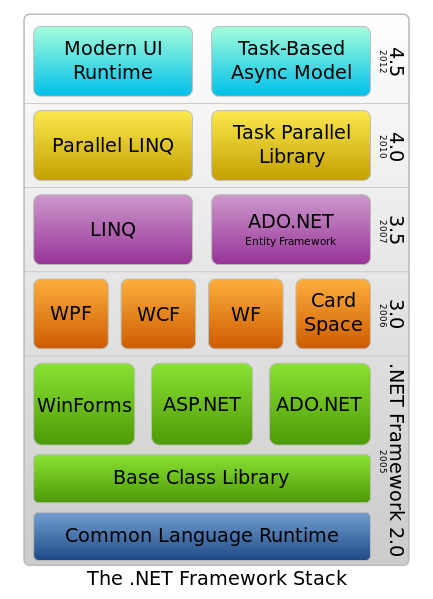
\includegraphics[scale=0.4]{DotNet.png}
\end{wrapfigure}
Die .NET-Plattform ist die Umsetzung des Common-Language-Infrastructure-Standards (CLI) und stellt mit diesem eine Basis zur Entwicklung und Ausführung von Programmen dar, die mit unterschiedlichen Programmiersprachen auf verschiedenen Plattformen erstellt wurden. Hauptbestandteile sind die (objektorientierte) Laufzeitumgebung Common Language Runtime (CLR), die Base Class Library (BCL) sowie diverse Hilfsprogramme zum Beispiel zur Rechteverwaltung. 
\subsubsection{CLR, CIL}
Die Common Language Runtime (CLR) ist die Laufzeitumgebung von .NET und stellt somit den Interpreter für den standardisierten Zwischencode, die Common Intermediate Language (CIL), dar. Die CIL hieß früher Microsoft Intermediate Language (MSIL), wurde aber im Rahmen der Standardisierung durch die Ecma International umbenannt. Für sie wurde ein sprachübergreifendes System von objektbasierten Datentypen definiert, so dass für alle Hochsprachen, die sich an den Common Language Infrastructure-Standard (CLI) halten, gültiger CIL-Bytecode erstellt werden kann. \\
.NET wurde von Anfang an dafür entwickelt, dass Programmierer in unterschiedlichen Programmiersprachen arbeiten können. Jede dieser Hochsprachen wird von .NET dann in die CIL übersetzt.
\subsubsection{Strategie, Nutzen und Trends}
Das Besondere an der CLR ist weniger die technische Innovation als vielmehr die strategische Entscheidung von Microsoft für ein laufzeitbasiertes System. Es soll unter anderem helfen, Systemabstürze zu vermindern, da die Runtime Applikationsfehler fangen kann. Damit entschied sich Microsoft erstmals gegen die bisher angewandte direkte Kompilierung in den Maschinencode des Zielsystems. Zusammen mit der Marktmacht von Java und dem Erfolg von Skriptsprachen ist damit ein Trend zu identifizieren. Dieser stellt einen Bruch mit den direktkompilierenden Programmiersprachen (insbesondere C++ und C) dar. \\
Mittels sog. „Reflection“ ist es möglich, zur Laufzeit Programmcode über ein Objektmodell zu generieren und es direkt im Speicher in lauffähigen Code zu überführen.
\subsubsection{Managed und Unmanaged}
Die .NET-Terminologie unterscheidet dabei zwischen Bytecode, welcher von der CLR verwaltet und in Maschinensprache umgesetzt wird – sogenannter Managed Code (v. engl. managed code ‚verwaltete Maschinensprache‘) –, und Teilen, die nicht innerhalb der CLR ausgeführt werden (unmanaged). Daneben gibt es noch die Möglichkeit in .NET unsicheren Code zu schreiben, um weiterhin z. B. klassische Zeiger-Operationen direkt auf einem Speicherbereich durchführen zu können. \\
Mit Hilfe der Interop-Technik lassen sich alle klassischen, binär kompilierten Windows-Bibliotheken mit .NET-Kapseln (sogenannten „Wrappern“) versehen und danach deren Programmfunktionen wie normale .NET Programmfunktionen aufrufen. Technisch gesehen gibt die CLR allerdings im Moment des Aufrufs einer Funktion einer nicht überwachten DLL einen großen Teil der Kontrolle über den Programmfluss ab. \\
Umgekehrt lassen sich auch .NET-Funktionen wie COM-Funktionen aufrufen. Damit soll eine fließende Migration von Software-Projekten auf .NET ermöglicht werden und die Integration von .NET-Modulen in eine bestehende Umgebung erleichtert werden.
\subsubsection{Sicherheit}
Eines der wichtigsten Konzepte von .NET ist die Sicherheit. Das Sicherheitskonzept beginnt bei Mechanismen, die die Identität des Programmherstellers gewährleisten sollen (Authentizität), geht über in solche zum Schutz der Programme vor Veränderung (Integrität) und reicht bis hin zu Techniken, die den Ort der Herkunft bzw. Programmausführung (zum Beispiel das Internet) einbeziehen. Es gibt sowohl ein codebasiertes (Code-based Security) als auch ein nutzerbasiertes (Role-based Security) Sicherheitsmodell.
\subsubsection{Attribute}
Eine programmiertechnisch interessante Neuerung von .NET ist die Einführung von Attributen: gekennzeichnete Metadaten als Bestandteil der Programmiersprache. Beispielsweise können im Rahmen der komponentenbasierten Programmierung Komponenteneigenschaften ausgedrückt werden. Für die Verteilung, Installation und Konfiguration, für die Sicherheit, für Transaktionen und andere Programme können dem Code beschreibende Eigenschaften hinzugefügt werden. \\
Innerhalb eines Programmes kann mit Hilfe von Reflection auf die Attribute eines .NET-Programms, Assembly genannt, und die in ihr enthaltenen Elemente zugegriffen werden.
\begin{center}
	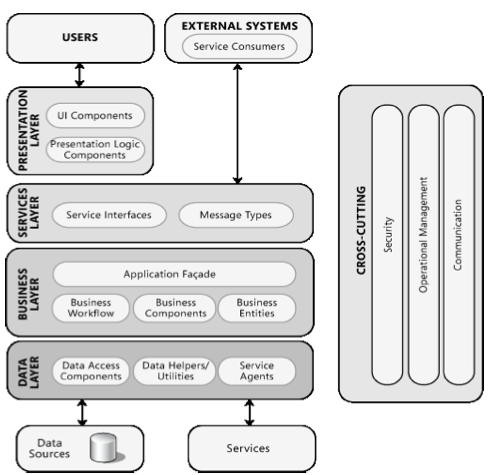
\includegraphics[scale=0.5]{enterprice_architecture.png}
\end{center}

\subsection{.NET Compact Framework}
Das .NET Compact Framework ist ein Teil des .NET-Frameworks, der speziell für die Nutzung auf mobilen Endgeräten wie beispielsweise Pocket-PCs, Smartphones und PDAs ausgerichtet ist. Es soll Entwicklern erleichtern, Anwendungen für mobile Geräte zu schreiben oder sie auf diese zu portieren. Microsoft wird so dem eigenen Anspruch auf Plattformunabhängigkeit, den sie mit dem .NET Framework verfolgen, noch etwas mehr gerecht. \\
Technisch gesehen ist das Compact Framework eine Laufzeitumgebung bzw. eine Klassenbibliothek (vgl. Framework). Diese Version ist gegenüber dem normalen .NET-Framework für den PC um eine größere Zahl von Klassen reduziert, die für Kleingeräte nicht benötigt werden oder zu viel Speicherplatz belegen.

\subsection{SharePoint}
SharePoint ist eine Webanwendung von Microsoft, die folgende Anwendungsgebiete abdeckt:
\begin{itemize}
	\item Zusammenarbeit, beispielsweise das Verwalten von Projekten oder die Koordination von Aufgaben,
	\item Soziale Netzwerke, beispielsweise über persönliche Webseiten, Team-Webseiten, Diskussionsgruppen und Blogs,
	\item Intranetportale,
	\item Content-Management über Dokumentenmanagement-Funktionen, Inhaltsverwaltung, Metadaten und benutzerangepasste Suchfunktionen,
	\item Geschäftsanwendungen.
\end{itemize}
\begin{center}
	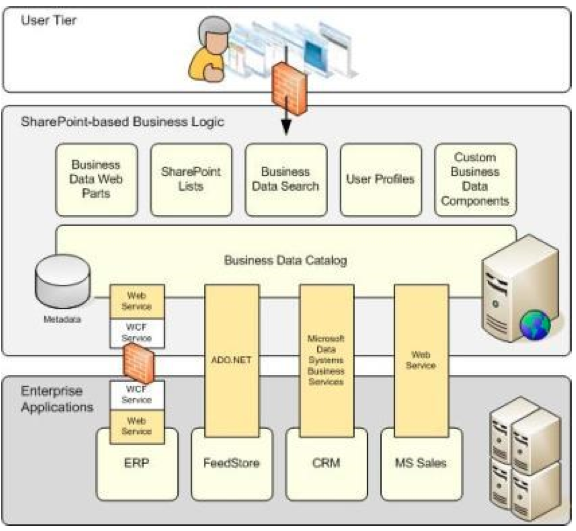
\includegraphics[scale=0.4]{sharepoint.png}
\end{center}

\subsection{BizTalk}
\begin{wrapfigure}{r}{0.3\textwidth}
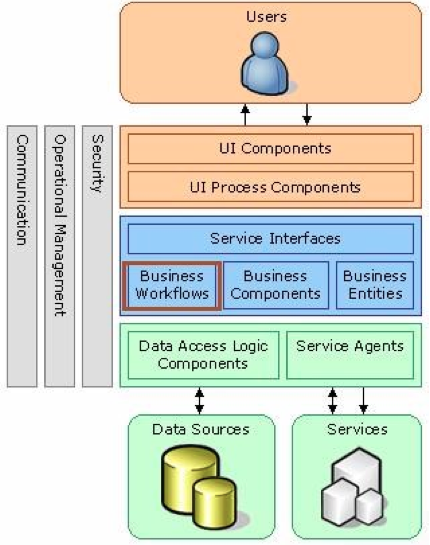
\includegraphics[scale=0.4]{bizzTalk.png}
\end{wrapfigure}
Microsoft BizTalk Server, oft einfach nur als „BizTalk“ bezeichnet, ist ein Enterprise Service Bus. Durch Adaptoren, die speziell darauf ausgelegt sind, in großen Unternehmen zwischen Systemen zu kommunizieren, wird eine Automatisierung von Geschäftsprozessen ermöglicht. Dieses Microsoft-Produkt enthält folgende Funktionen: Enterprise Application Integration (EAI), Business Process Automation, Business-to-business Communication, Message broker, and Business Activity Monitoring. \\
Im Standardfall ermöglicht BizTalk Firmen durch den Austausch von Geschäftsdokumenten, wie Bestellungen und Rechnungen zwischen zwei getrennten Applikationen, automatisierte Geschäftsprozesse zu integrieren und zu verwalten. Das ist innerhalb einer Organisation sowie über Unternehmensgrenzen hinweg möglich. Auf Anwender bezogene Prozesse können nicht direkt mit BizTalk implementiert werden. Das dafür entsprechende Microsoft-Produkt wäre hier der Microsoft-Sharepoint-Server. \\
Die Entwicklung für BizTalk erfolgt durch Microsoft Visual Studio. Ein Entwickler kann „Transformations Maps“ erzeugen, die einzelne Nachrichtentypen in andere verwandelt. Beispielsweise kann eine XML Datei in ein SAP-IDocs-Format übersetzt werden. Diese Maps können in Visual Studio mit einem grafischen Designer erstellt werden. Weitere Funktionalität kann über .NET Assemblies bereitgestellt werden, die von bestehenden Modulen, wie „Instance Maps“ oder Adaptoren aufgerufen werden können. Datentransformationen (Maps) und auch Prozesse ist durch sogenannte „Orchestrierungen“" organisiert, die eine Visualisierung des Prozesses ermöglicht.

\subsection{Summary}
\begin{itemize}
	\item The .Net Framework includes \textbf{MS proprietary frameworks} for application development
	\item The application development frameworks are \textbf{not ECMA/ISO standard }
	\item Microsoft offers many \textbf{additional components} for Enterprise Application Development. Often still not .Net technology
	\item The \textbf{Microsoft Application Architecture Guide} describes reference archictectures for different enterprise application scenarios.
\end{itemize}

\pagebreak
\section{Team Foundation Server}
Der Team Foundation Server (TFS) von Microsoft ist eine Windows-Plattform für kollaborative Softwareprojekte. Über den TFS können Projekte geplant, erstellt und verwaltet werden. Er kann dabei bis zu 2000 Entwickler und 500 Projekte verwalten.[ Für kleine Projekte gibt es die Workgroup-Edition, die maximal fünf Benutzer erlaubt. \\
Auf Basis der Prozessvorlagen unterstützt der TFS verschiedene Entwicklungsverfahren. Vorlagen für die Standardverfahren CMMI, Agile Softwareentwicklung oder Scrum werden mitgeliefert. Andere Hersteller bieten weitere Prozessvorlagen an. Alle Prozessvorlagen liegen in Form von XML-Dateien vor, so dass grundsätzlich ein (XML-)Editor für deren Bearbeitung ausreicht. Für eine einfachere und schnellere Anpassung steht allerdings ein Werkzeug zur Verfügung, mit dem die Anpassungen direkt in der Entwicklungsumgebung vorgenommen werden können. Die beim Prozess mitgelieferte Dokumentation („Process Guidance“) liegt statisch vor, kann aber dank verfügbaren Quelldateien angepasst und neu erstellt werden. \\
Die involvierten Teammitglieder können mit verschiedenen Werkzeugen (zum Beispiel Visual Studio, Excel, Project, Infopath, Office, Outlook oder Web) Prozessschritte bearbeiten und die entsprechenden Arbeitsschritte ("workflows") anstoßen. Die genannten Programme integrieren sich direkt in den TFS, so dass auf einer einheitlichen Plattform gearbeitet werden kann. \\
Bestandteile einer Prozessvorlage sind Work Items, Reports, Abfragen und diverse Dokumente.
\begin{center}
	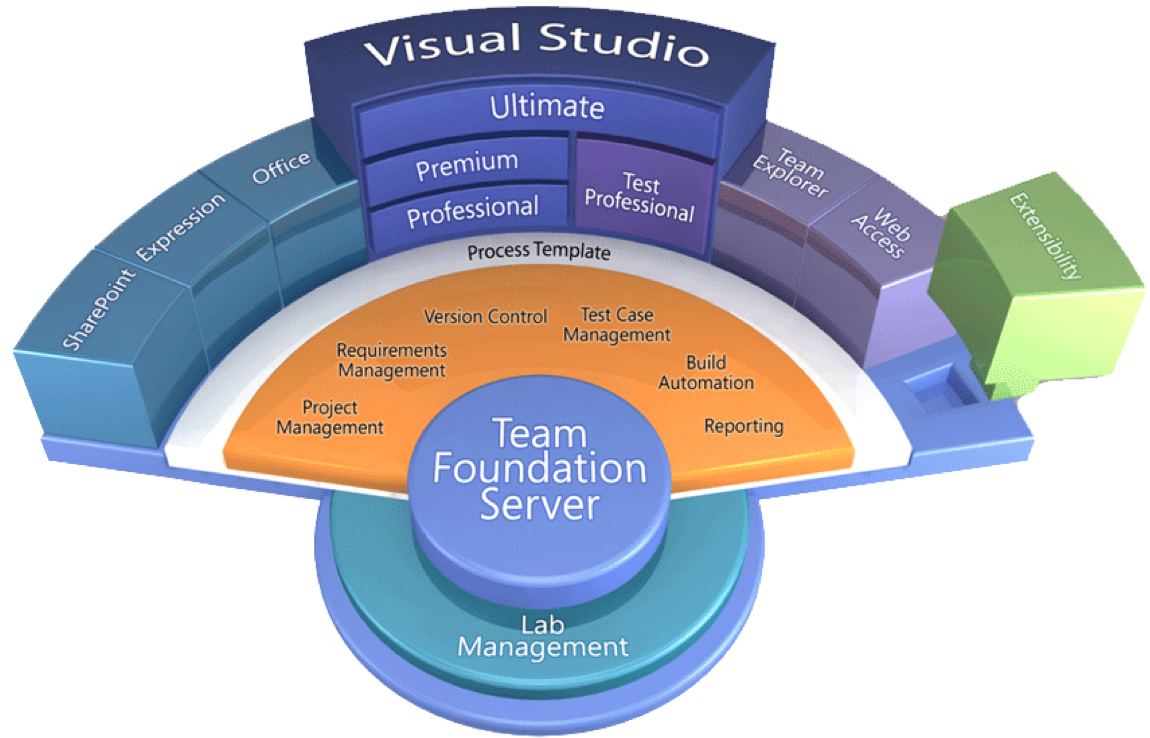
\includegraphics[scale=0.2]{tfs.png}
\end{center}
\subsection{Features}
\subsubsection{Versionskontrolle}
TFS integriert eine eigene Versionskontrolle für den Quellcode der verwalteten Projekte. Die gängigen Operationen eines Versionskontrollsystems werden unterstützt.
\subsubsection{TFS-Build}
Die Buildengine des TFS unterstützt das automatische Erstellen des entwickelten Produkts ("build"), optional z.B. auch mit Dokumentation. Dabei kann man auch Unittests ausführen und Statistiken bzw. Berichte generieren lassen.
\subsubsection{Reports}
Über ein integriertes Data-Warehouse werden automatisch Berichte erstellt (etwa mit Metriken, Fehlerstatistik, Leistungsanalyse usw.) Die Berichte sind für unterschiedliche Zielpersonen zugeschnitten (Kostenverantwortliche, Entwickler, Projektleiter) und geben jeweils einen Überblick über den Projektstand. Technische Grundlage ist ein sogenannter "report server", der seine Ausgabe über einen Microsoft SharePoint Server generiert. Dadurch können die Berichte sowohl direkt als auch in Microsoft Project, Microsoft Excel und innerhalb von Microsoft Visual Studio benutzt werden.
\subsubsection{Benutzerverwaltung}
Der TFS kann entweder als Server in einem Active Directory oder einzeln betrieben werden. Für die Benutzerverwaltung kennt der Server die Windows-Benutzer und Gruppen sowie weitere Gruppen im TFS. Beim Anlegen eines Projekts werden vier Gruppen automatisch erstellt: Lesezugriff, Schreibzugriff, Administratoren und eine interne Gruppe zum Buildmanagement. \\
Die Berechtigungen für den "Sharepoint Server" sowie das "reporting system" müssen vom Administrator von Hand gesetzt werden. Aus diesem Grund empfiehlt es sich, Windows-Gruppen zu definieren und zu verwenden.
\subsubsection{Serveraufbau}
Der TFS ist auf dem Prinzip einer Schichtenarchitektur entwickelt worden. Anwendungs- und Datenschicht können auf einem einzelnen Server oder auf separaten Servern installiert werden. \\
Der TFS benötigt folgende Software:
\begin{itemize}
	\item Microsoft SQL Server für die Datenhaltung und das Data-Warehouse (x86 oder x64)
	\item Windows Server 2003, Windows Server 2008 für die Anwendung (x86 oder x64)
	\item TFS-Build entweder integriert oder separat
	\item Microsoft Internet Information Server und Windows SharePoint Services
	\item Microsoft Report Server
\end{itemize}
Ab der Version 2010 kann der Team Foundation Server auch auf einem Client-Betriebssystem installiert werden. Hierfür wird eine Basis-Konfiguration angeboten, welche die Express-Version des Microsoft SQL Servers zur Datenhaltung benutzt. Diese Installationsform ist für Einzelentwickler gedacht, die den Team Foundation Server benutzen wollen. Microsoft möchte hierdurch den Team Foundation Server als Nachfolger des Produkts Microsoft Visual SourceSafe etablieren, welches nicht mehr von Microsoft gepflegt wird. \\
Die einzelnen Komponenten, mit Ausnahme des Windows-Server-Betriebssystems und des SQL Servers, sind Bestandteil des Produkts.

\pagebreak
\section{Windows Presentation Foundation}
Windows Presentation Foundation (kurz WPF), auch bekannt unter dem Codenamen Avalon, ist ein Grafik-Framework und Teil des .NET Frameworks von Microsoft, das mit Windows Vista, Windows 7 und Windows 8 ausgeliefert wird, sich aber auf Windows XP (bis zur Version 4.0) und Server 2003 nachinstallieren lässt. \\
WPF stellt ein umfangreiches Modell für den Programmierer bereit. Dabei werden die Präsentation und die Geschäftslogik getrennt, dies wird vor allem durch die Auszeichnungssprache XAML (basierend auf XML) unterstützt. XAML beschreibt Oberflächen-Hierarchien deklarativ als XML-Code. WPF-Anwendungen können sowohl Desktop- als auch Web-Anwendungen sein und benutzen, wenn möglich, auch Hardwarebeschleunigung. Das Framework versucht, die verschiedenen Bereiche, die für die Präsentation wichtig sind (Benutzerschnittstelle, Zeichnen und Grafiken, Audio und Video, Dokumente, Typographie), zu vereinen.
\begin{center}
	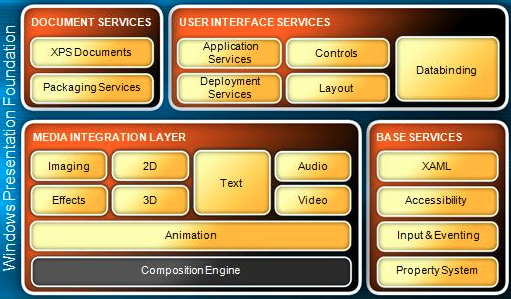
\includegraphics[scale=0.6]{wpf_architecture.png}
\end{center}
\subsection{Leistungsmerkmale}
\subsubsection{Eigenschaften und Ereignisse}
Im Gegensatz zu normalen Anwendungen benutzt WPF eine eigene Art von Eigenschaften, dependency properties genannt. Diese sind notwendig, da in WPF einige Eigenschaften von anderen abhängig sein können, z. B. die Position eines Bilds während einer Animation. Zudem bieten diese Eigenschaften Unterstützung für Datenbindung und Validierung. \\
Auch die Ereignisse unterscheiden sich. In WPF werden so genannte routed events benutzt. Dies ergibt sich daraus, dass Elemente andere Elemente enthalten können. Wenn ein Kindelement ein Ereignis auslöst, so wird dieses auch an das Elternelement geleitet, um nicht jedes einzelne Kindelement zu überwachen. Dies nennt sich bubble event. Umgekehrt kann es sinnvoll sein, ein Ereignis als Elternelement vor dem Kindelement zu empfangen (tunnel event). \\
Dependency properties und routed events können auch attached sein, d. h. ein Element kann je nach Kontext eine Eigenschaft bzw. ein Ereignis von einem anderen Element erhalten. Dies ist z. B. der Fall, wenn eine Schaltfläche in einem Raster steckt: es werden Eigenschaften für die Positionierung (Spalte und Zeile) zur Verfügung gestellt.
\subsubsection{Grafik}
Alle Grafikelemente (auch Fenster, etc.) werden via Direct3D gerendert.[1] Dies hat zur Folge, dass einige Aufgaben hardwarebeschleunigt von der GPU der Grafikkarte übernommen werden anstatt von der CPU. Zudem können 3D-Grafiken in 2D-Anwendungen angezeigt werden. Auch Vektorgrafiken werden unterstützt. Bis zur Version 3.5 der WPF werden Bitmap-Effekte angeboten, diese werden allerdings ohne Hardwarebeschleunigung gerendert,[2] weshalb sie in der aktuellen Version 4.0 als veraltet deklariert werden. Anstelle der Bitmap-Effekte sollen nun "normale" Effekte wie z. B. der DropShadowEffect verwendet werden, welche durchgängig die Hardwarebeschleunigung der Grafikkarte verwenden.
\subsubsection{Interoperabilität}
Windows-Forms-Steuerelemente können in WPF-Anwendungen benutzt werden; umgekehrt können auch WPF-Elemente in Windows Forms gehostet werden. \\
Zudem unterstützt WPF Win32: WPF ist mittels Hosting auch in Win32-Code benutzbar und Win32-Code kann auch in WPF-Anwendungen weiterbenutzt werden.
\subsubsection{Medien und Dokumente}
WPF stellt 2D-Primitive mit vordefinierten Transformationen, Texturen, etc. bereit. Die 3D-Funktionalitäten sind ein Unterteil von Direct3D. Diese Funktionalitäten sind allerdings auch für Dokumente und Benutzerschnittstellen verfügbar. \\
Auch individuelle Animationen sind möglich. Diese können auch zeitgesteuert ablaufen.
Die meisten Grafikformate und Videos im WMV oder MPEG-Format werden unterstützt, wobei hierfür ein installierter Windows Media Player ab Version 9 notwendig ist. \\
Auch Dokumente, insbesondere XPS-Dokumente werden mit vordefinierten Steuerelementen unterstützt.
\subsubsection{Text und Typographie}
WPF unterstützt viele Features von OpenType, z. B. Ligaturen, Kapitälchen und Ruby. Es werden OpenType- und TrueType-Schriftarten unterstützt. WPF behandelt Text, da es auf .NET aufsetzt, immer als Unicode unabhängig von der Zeichenkodierung.
\subsubsection{Benutzerschnittstelle}
WPF enthält schon einige vordefinierte Steuerelemente, wie Menüs, Listen, etc. \\
Zudem wird das Aussehen von der Steuerelementlogik getrennt. Das Aussehen eines Steuerelements kann unabhängig davon mit Styles (Eigenschaften anpassen) und Templates (Festlegung, wie das Steuerelement aufgebaut ist) geändert werden. \\
Steuerelemente können beliebige andere Steuerelemente oder Inhalte (z. B. Bilder) enthalten.
\subsection{XAML}
\begin{itemize}
	\item e\textbf{X}tensible \textbf{A}pplication \textbf{M}arkup \textbf{L}anguage
	\item XML based language to instantiate and initialize Objects with hierarchical relationships
	\item Also used in WF (Workflow Foundation) und Silverlight
\end{itemize}
\begin{lstlisting}[language=Java, caption=xaml, style=JavaStyle]
<Window xmlns="http://schemas.microsoft.com/winfx/...">
	<StackPanel HorizontalAlignment="Center" >
		<Image Source="Images/hello.jpg" Height="80" />
		<TextBlock Text="Welcome to WPF!" FontSize="14"/>
		<Button Content="OK" Padding="10,4" />
	</StackPanel>
</Window>
\end{lstlisting}
\subsubsection{Declarative Programming}
Markup for Windows
\begin{itemize}
	\item Build applications in simple declarative statements
	\item Can be used for any CLR object hierarchy (not just WPF)
\end{itemize}
Code and content are strictly separate
\begin{itemize}
	\item Streamline collaboration between designers and developers
\end{itemize}
\subsubsection{XAML vs. Code}
\begin{itemize}
	\item What can be done in XAML can also be done in code
	\item  XML-Tags correspond to objects (using the default constructor)
	\item XML-Attributes correspond to properties
\end{itemize}
\begin{lstlisting}[language=Java, caption=XML, style=JavaStyle]
<StackPanel HorizontalAlignment="Center" >
	<TextBlock Margin="20">Hello</TextBlock>
</StackPanel>
\end{lstlisting}
\begin{lstlisting}[language=Java, caption=C\#, style=JavaStyle]
StackPanel stackPanel = new StackPanel();
TextBlock textBlock = new TextBlock();
textBlock.Margin = new Thickness(10);
textBlock.Text = "Welcome to WPF";
stackPanel.Children.Add(textBlock);
\end{lstlisting}
\subsubsection{Namespaces}
XML-Prefixes correspond to CLR-Namespaces
\begin{lstlisting}[language=Java, caption=Namespaces, style=JavaStyle]
<Window xmlns=http://schemas.microsoft.com/winfx/2006/xaml/presentation xmlns:x="http://schemas.microsoft.com/winfx/2006/xaml" xmlns:cc="clr-namespace:MyCoolControls">
    <Grid>
        <cc:MyControl x:Name="myControl" />
    </Grid>
 </Window>
\end{lstlisting}
\subsubsection{Property Element Syntax}
Complex properties can be defined as XML child elements
\begin{lstlisting}[language=Java, caption=Property Element Syntax, style=JavaStyle]
<Rectangle Fill="Red" />

<Rectangle Width="20" Height="20">
	<Rectangle.Fill>
		<LinearGradientBrush>
			<GradientStop Color="Red" Offset="0" />
			<GradientStop Color="Blue" Offset="1" />
		</LinearGradientBrush>
	</Rectangle.Fill>
</Rectangle>
\end{lstlisting}
\subsection{XAML compilation}
\begin{center}
	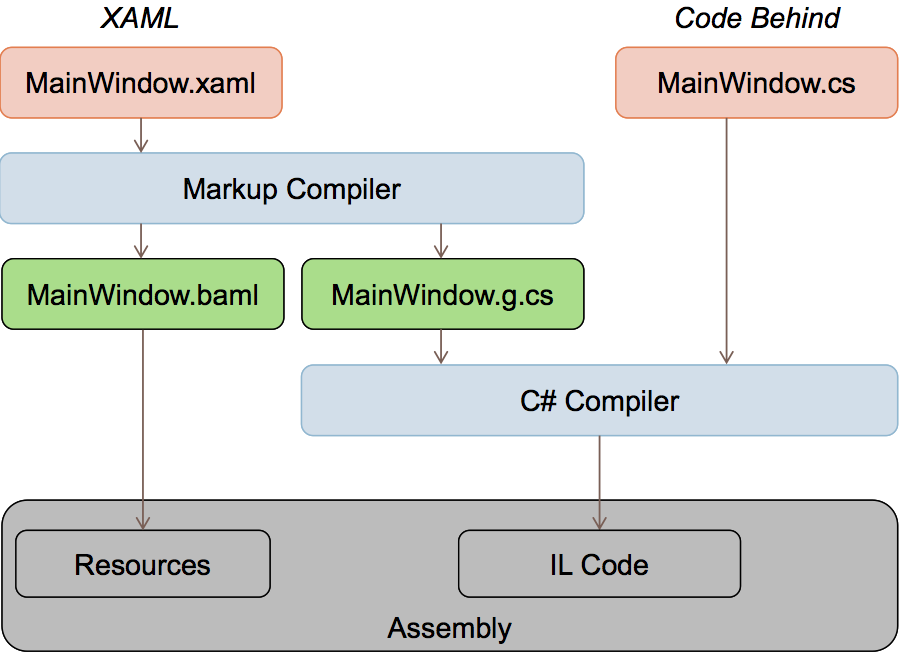
\includegraphics[scale=0.2]{xaml_compilation.png}
\end{center}
\subsection{XAML Layout}
\subsubsection{Panels}
\begin{center}
	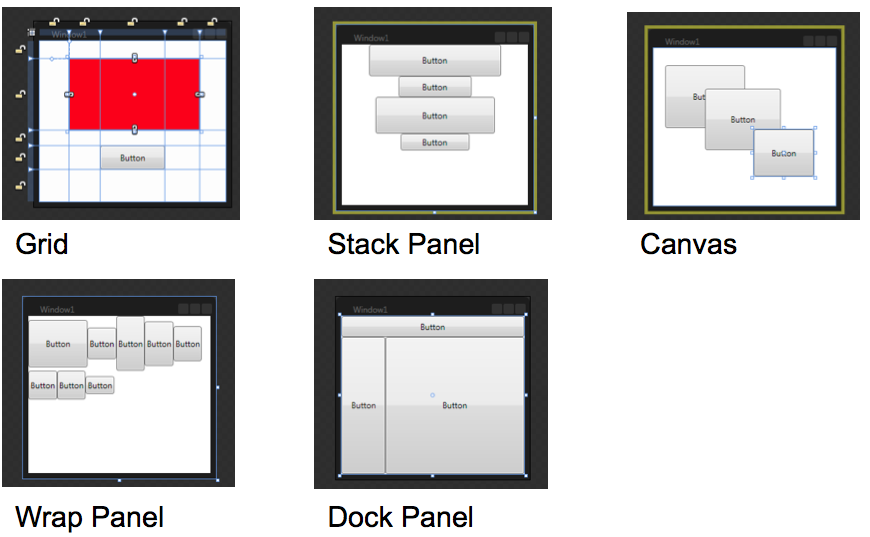
\includegraphics[scale=0.2]{xaml_panels.png}
\end{center}
\subsubsection{Attached Properties}
Attached Properties allow to add properties to WPF Controls
\begin{lstlisting}[language=Java, caption=Attached Properties, style=JavaStyle]
<DockPanel>
	<Button DockPanel.Dock="Left" Content="Button" />
</DockPanel>

<Canvas>
	<Button Canvas.Top="20" Canvas.Left="20" Content="Button" />
</Canvas>
\end{lstlisting}
\subsubsection{Margin, Padding und Alignment}
\begin{center}
	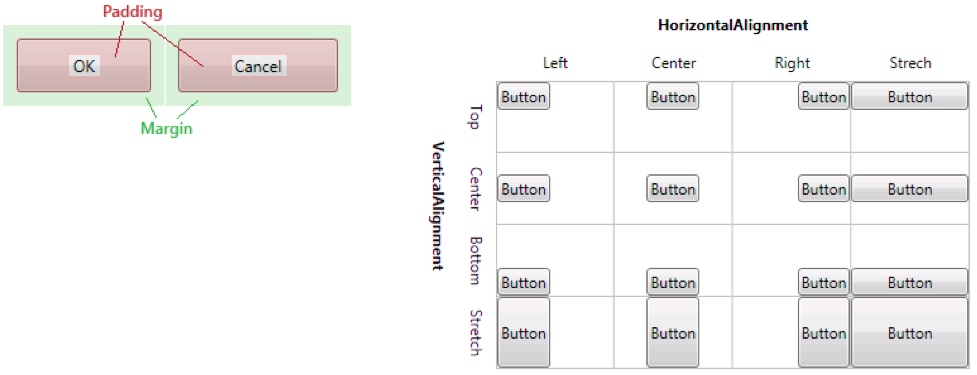
\includegraphics[scale=0.3]{xaml_alignement.png}
\end{center}
\begin{lstlisting}[language=Java, caption=Alignment, style=JavaStyle]
<Button HorizontalAlignment="Left" VerticalAlignment="Top" Margin="8,0,8,8" >
    Test
</Button>
\end{lstlisting}
\subsubsection{Transformation}
\begin{itemize}
	\item Element can be transformed in WPF
	\item LayoutTransform influences the layout, RenderTransform does not
\end{itemize}
\begin{center}
	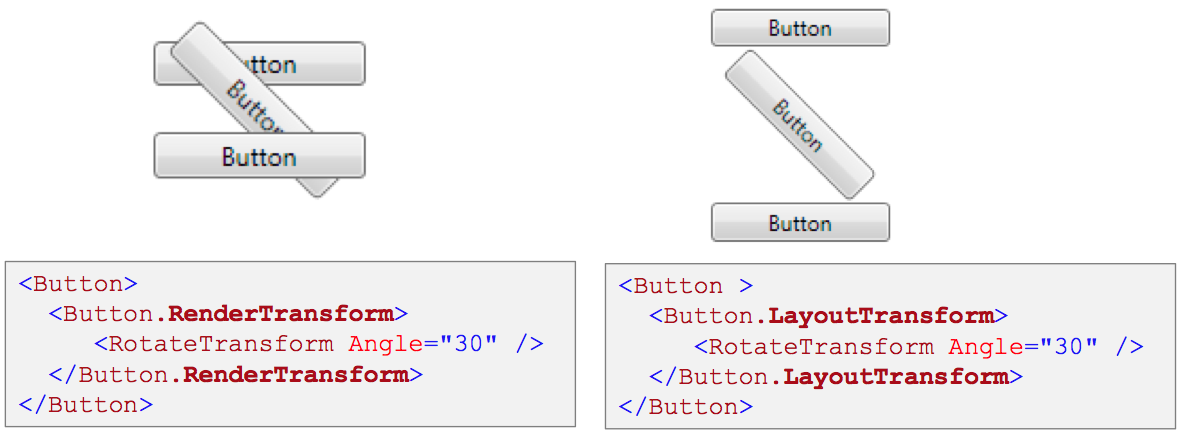
\includegraphics[scale=0.3]{xaml_rendering.png}
\end{center}
\subsection{Data Binding}
Markup Extensions are a kind of XAML- Macros, resolved at runtime.
\begin{lstlisting}[language=Java, caption=Data Binding, style=JavaStyle]
<TextBlock Text="{Binding Path=Vorname}" />
\end{lstlisting}
\begin{itemize}
	\item DataBinding synchronizes the values of two properties
	\item Typically a UI element is connected to an entity object from a datasource, e.g. the database
	\item Uni- oder bidirectional
	\item A ValueConverter can adapt the data format
\end{itemize}
\begin{center}
	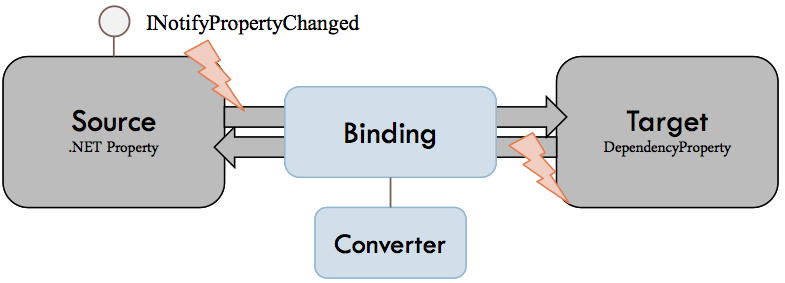
\includegraphics[scale=0.25]{xaml_dataBinding.png}
\end{center}
\begin{lstlisting}[language=Java, caption=Sources Data Binding, style=JavaStyle]
// Other WPF elements
{Binding Path=Text, ElementName=textBox}

// Parent WPF elements
{Binding Path=Text, RelativeSource={RelativeSource Mode=FindAncestor, AncestorType=ListBox}}

//Explicit Objekts
{Binding Path=Text Source={StaticResource myObject}}

//DataContext
 {Binding Path=Text}
\end{lstlisting}
\subsubsection{DataContext}
\begin{itemize}
	\item Every WPF element has a DataContext property
	\item The DataContext is inherited to children
	\item Allows the Binding to a Data-Object
	\item The default source of a \{Bindings\} is always the DataContext
\end{itemize}
\subsubsection{UpdateTrigger \& Binding Direction}
\begin{description}
	\item[UpdateSourceTrigger] Defines when is the DataBinding is triggered:
		\begin{itemize}
			\item PropertyChanged
			\item LostFocus
			\item Explicit
		\end{itemize}
	\item[Mode] Defines the DataBinding direction:
		\begin{itemize}
			\item OneWay
			\item TwoWay
			\item OneWayToSource
		\end{itemize}
\end{description}
\subsubsection{INotifyPropertyChanged}
Every Data-Object must implement INotifyPropertyChanged to allow the
propagation of changes:
\begin{lstlisting}[language=Java, caption=INotifyPropertyChanged, style=JavaStyle]
public class Customer : INotifyPropertyChanged {
	private string _name;
	public string Name {
		 get { return _name; }
		set {
			_name = value;
			NotifyPropertyChanged("Name");
		}
	}
	public event PropertyChangedEventHandler PropertyChanged;
	private void NotifyPropertyChanged( string name) {
		if( PropertyChanged != null )
			PropertyChanged(this, new PropertyChangedEventArgs(name));
	}
}
\end{lstlisting}
\subsubsection{ObservableCollection}
Use ObservableCollections to allow the propagation of collection changes:
\begin{lstlisting}[language=Java, caption=ObservableCollection, style=JavaStyle]
ObservableCollection<Auction> auctions = new ObservableCollection<Auction>();
\end{lstlisting}

\subsection{Value Converter}
ValueConverters can change the format of the data in both directions:
\begin{lstlisting}[language=Java, caption=Value Converter, style=JavaStyle]
public class BoolToVisibilityConverter : IValueConverter {
	#region IValueConverter Members
	public object Convert(object value, Type targetType, object parameter, CultureInfo culture) {
		return (bool) value ? Visibility.Visible : Visibility.Collapsed;
	}
	public object ConvertBack(object value, Type targetType, object parameter,  CultureInfo culture) {
		throw new NotImplementedException();
	}
	#endregion
}	
\end{lstlisting}
How to use a ValueConverter as a Resource in XAML:
\begin{lstlisting}[language=Java, caption=Value Converter, style=JavaStyle]
<Window.Resources>
	<conv:BooleanToStatusTextConverter x:Key="booleanToStatusTextConverter" />
</Window.Resources>
<Button Content="{Binding IsOpen, Converter={booleanToStatusTextConverter}}" />
\end{lstlisting}

\pagebreak
\section{Model-View-ViewModel}
\subsection{Einleitung}
\begin{itemize}
	\item \textbf{Separation of GUI design (\"{}style“) and logic "behavior" }\\ Ability to use Expression Blend
	\item \textbf{No duplicated code to update views} \\ No "myLabel.Text = newValue" sprinkled in code behind everywhere.
	\item \textbf{Testability: }\\ Since your logic is completely agnostic of your view (no "myLabel.Text" references), unit testing is made easy.
\end{itemize}
Each View binds to a single ViewModel that provides all functionality and data
\begin{itemize}
	\item Makes the ViewModel unit-testable
	\item Simplifies the data binding
\end{itemize}
\subsubsection{Pattern}
\begin{center}
	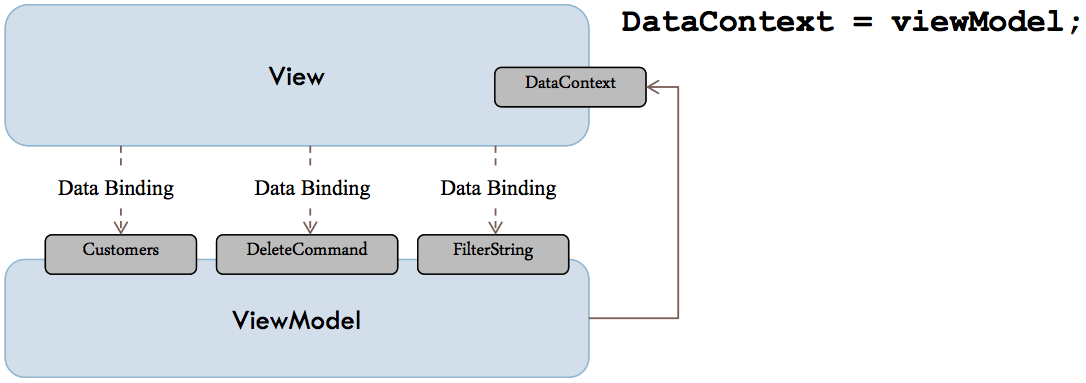
\includegraphics[scale=0.2]{mvvm_pattern.png}	
\end{center}
\subsubsection{User Interaction}
\begin{center}
 	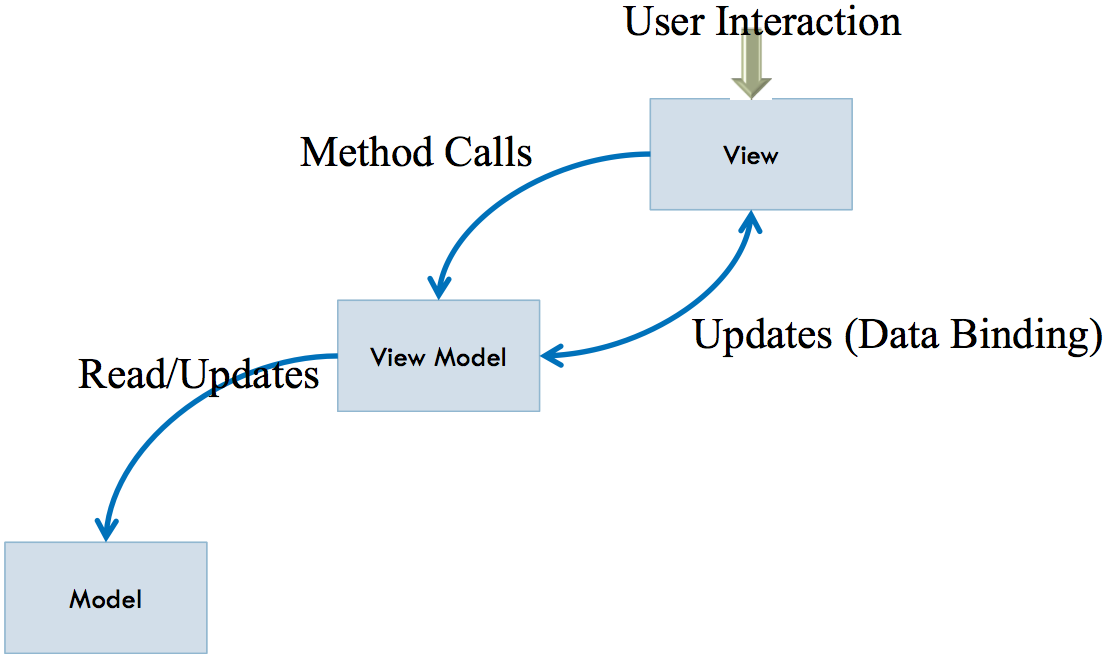
\includegraphics[scale=0.2]{mvvm_interaction.png}
\end{center}
\subsubsection{Overview}
\begin{center}
 	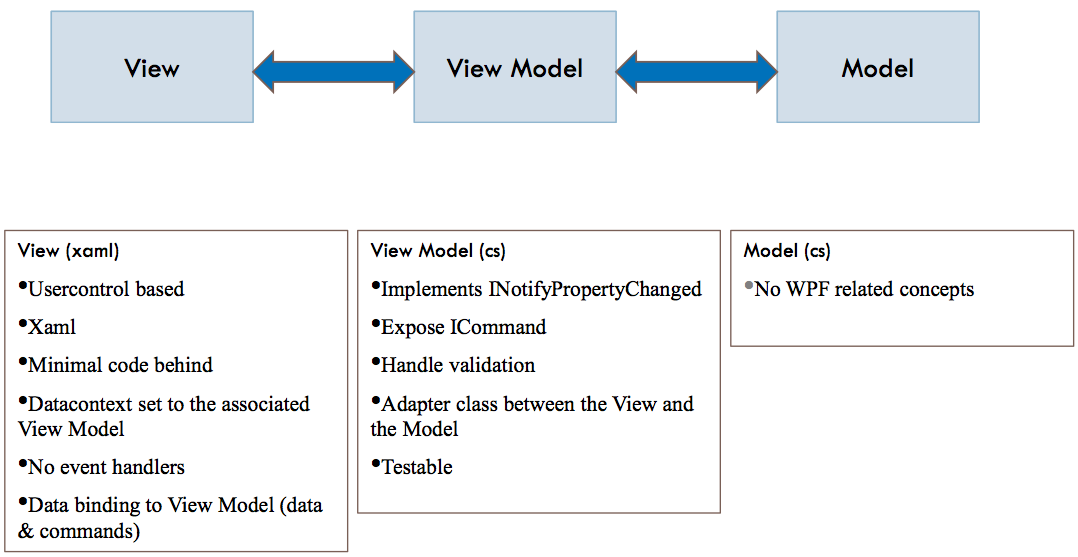
\includegraphics[scale=0.2]{mvvm_overview.png}
\end{center}

\subsection{Commands}
Commands are used to bind UI actions to the ViewModel functionality. A Command implements the following 3 functions of the ICommand Interface:
\begin{itemize}
	\item Execute(object param);
	\item CanExecute(object param);
	\item event CanExecuteChanged;
\end{itemize}
Commands can be used on different UI Elements (Button, Menu, KeyboardShortcut). \\
To use commands in the ViewModel you have to implement your own generic command class:
\begin{lstlisting}[language=Java, caption=Commands:, style=JavaStyle]
public class FooCommand : ICommand  {
	public Action<object> ExecuteDelegate { get; set; }
	public Func<object, bool> CanExecuteDelegate { get; set; }
	
	#region ICommand Members
	public bool CanExecute(object parameter) {
		return CanExecuteDelegate(parameter);
	}

	public event EventHandler CanExecuteChanged;
	
	public void Execute(object parameter) {
		ExecuteDelegate(parameter);
	}
	#endregion
}
\end{lstlisting}

\pagebreak
\section{Entity Framework}
\subsection{ADO.NET}
\subsubsection{Architecture}
\begin{center}
	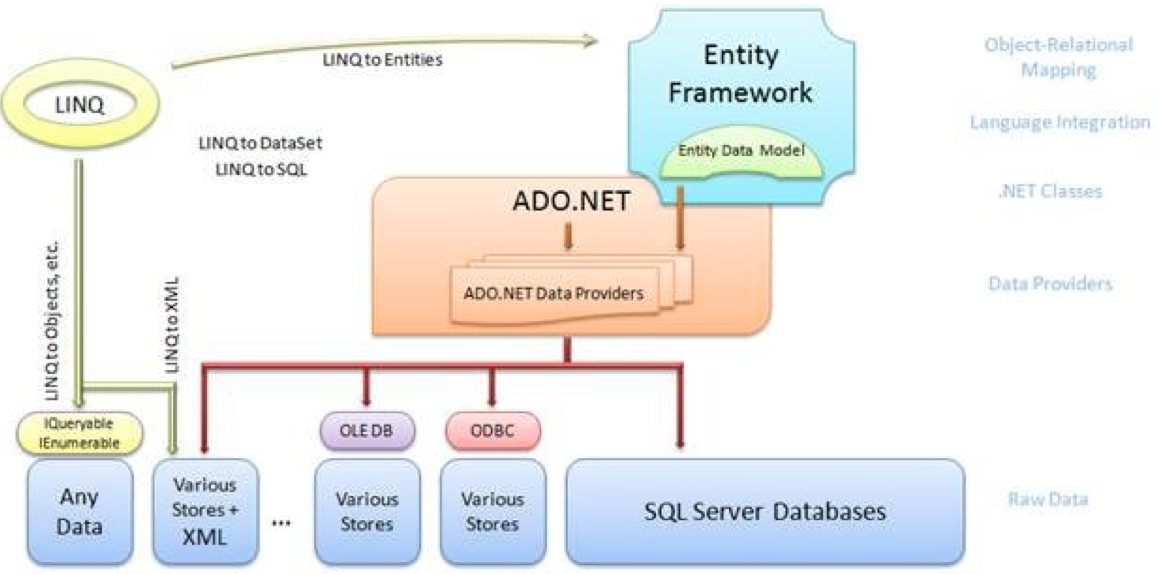
\includegraphics[scale=0.25]{ado_architecture.png}
\end{center}
\subsubsection{Data Provider}
\begin{center}
	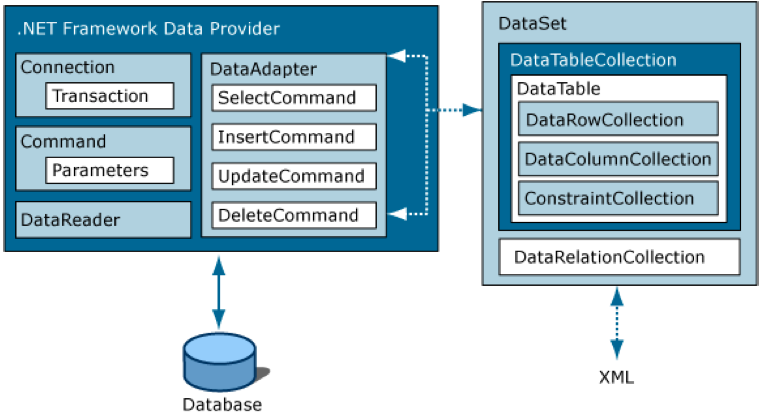
\includegraphics[scale=0.4]{ado_data_provider.png}
\end{center}
\subsection{Considerations}
\begin{itemize}
	\item Low level, full control
	\item Connected or disconnected
	\item You are responsible for entity mapping
	\item Flexible, high performance
\end{itemize}
$\rightarrow$ ADO.NET is the basis for other data access technologies and is going to stay
\subsubsection{Sample}
\begin{lstlisting}[language=Java, caption=Sample:, style=JavaStyle]
using (SqlConnection conn = new SqlConnection("<connection string>")) {
	conn.Open();
	SqlCommand cmd = new SqlCommand("select * from products", conn);
	using (SqlDataReader rd = cmd.ExecuteReader()) {
		while (rd.Read() {
			Console.WriteLine(rd["ProductName"]);
		}
	}
}
\end{lstlisting}
\begin{lstlisting}[language=Java, caption=DataSet Sample:, style=JavaStyle]
using (SqlConnection cn = new SqlConnection("<connection string>") {
	cn.Open();
	SqlDataAdapter ad = new OleDbDataAdapter("select * from products", cn); 
	DataSet ds = new DataSet();
	ad.Fill(ds, "Products");
	foreach(DataRow dr in ds.Tables["Products"].Rows) {
		Console.WriteLine(dr["ProductName"]);
	}
}
\end{lstlisting}
\subsubsection{the base for ORMs}
\begin{itemize}
	\item ADO.NET Entity Framework (EF)
	 \begin{itemize}
	 	\item Maps conceptual model to physical tables
	 	\item LINQ
	 \end{itemize}
	 \item LINQ to SQL
	 \begin{itemize}
	 	\item Lightweight, no mapping
	 	\item Replaced by EF but still supported by MS
	 \end{itemize}
	 \item NHibernate
	 \begin{itemize}
	 	\item Open Source
	 	\item LINQ
	 \end{itemize}
	 \item 3rd Party O/RMs
	 \begin{itemize}
	 	\item Telerik OpenAccess \& others
	 \end{itemize}
\end{itemize}
\subsection{Entity Framework}
\subsubsection{Overview}
\begin{itemize}
	\item Object / Relational Mapping
	\item LINQ as query language
	\item Features like: change tracking, identity resolution, lazy loading, etc.
\end{itemize}
\begin{center}
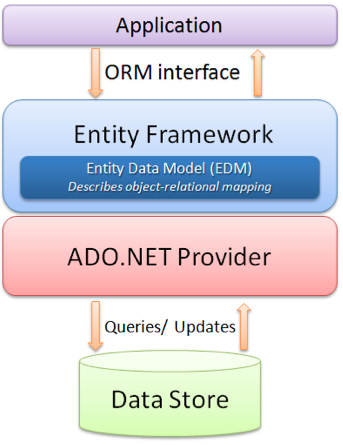
\includegraphics[scale=0.3]{ef_overview.png}
\end{center}
\subsubsection{Architecture}
\begin{center}
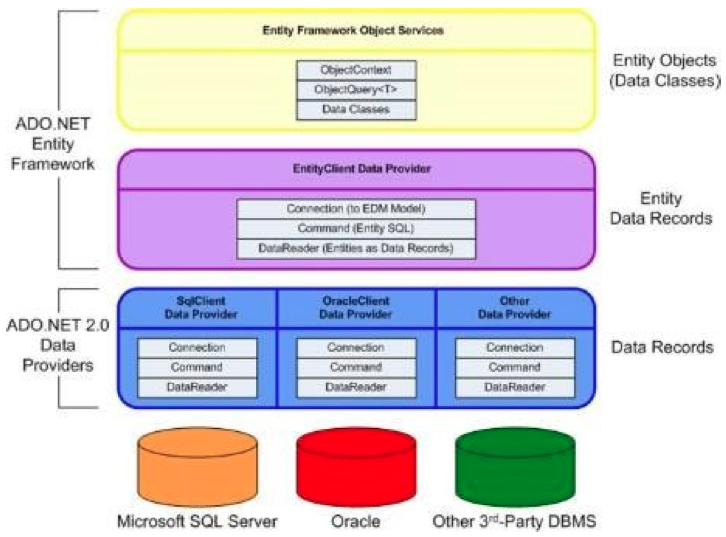
\includegraphics[scale=0.4]{ef_architecture.png}
\end{center}
\subsubsection{Entity Data Model}
\begin{center}
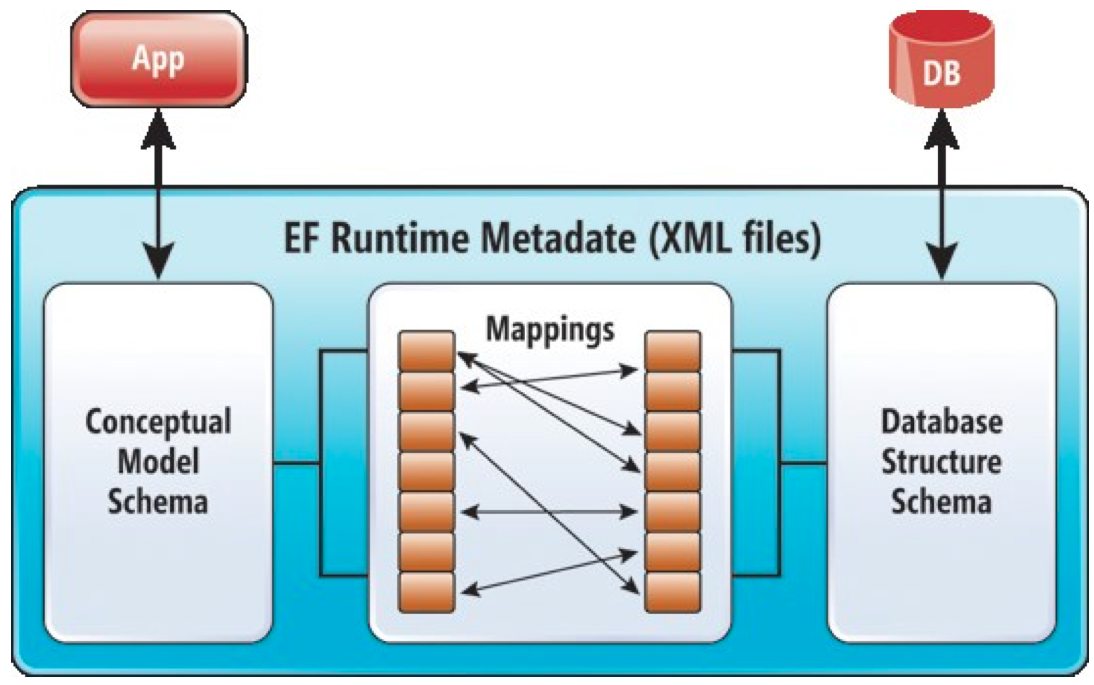
\includegraphics[scale=0.2]{entity_data_model_1.png}
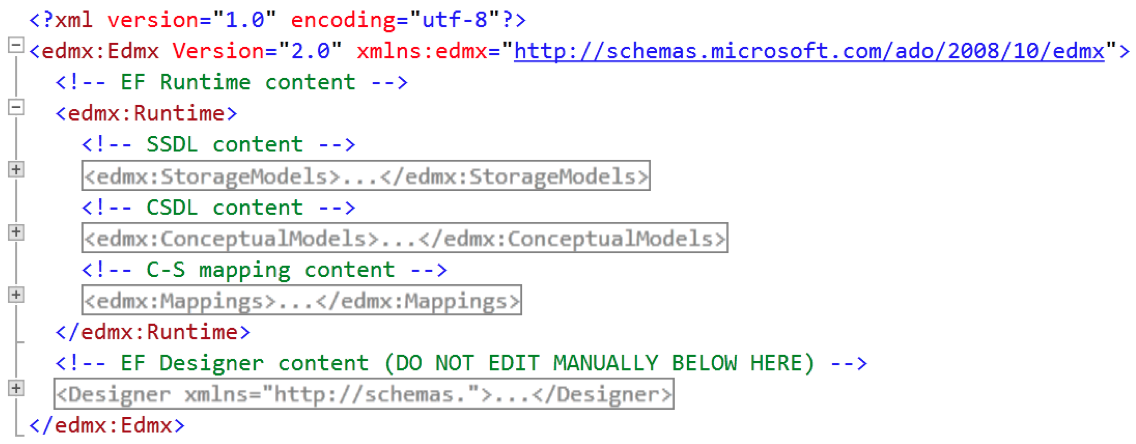
\includegraphics[scale=0.4]{entity_data_model_2.png}
\end{center}
\subsubsection{Benefits \& Considerations}
\begin{itemize}
	\item Decouples logical model from database model
	\item Consistent, independent query language
	\item Rich designer support
	\item Most common patterns (1-to-many, many-to-1, many-to-many, self-referencing, inheritance,
	\item Slower than ADO.NET core
	\item Must regenerate EDM after DB changes
\end{itemize}

\pagebreak
\section{Dependency Injection}
\subsection{DI and IoC}
\subsubsection{Overview}
\begin{itemize}
	\item Higher level modules should not depend on lower level modules
	\item Both should depend on abstractions (Interfaces or Abstract classes)
	\item Abstractions should not depend on details
\end{itemize}
\subsubsection{Implications}
\begin{itemize}
	\item Layers / Modularization
	\item Interface based programming
	\item Separated Interface (put interface in separate package than implementation)
	\item Implementation through Dependency Injection, for example
\end{itemize}
\subsubsection{Advantages of IoC}
\begin{itemize}
	\item Increase loose coupling
	\begin{itemize}
		\item Abstract interfaces don't change
		\item Concrete classes implement interfaces
		\item Concrete classes easy to throw away and replace
	\end{itemize}
	\item Increase mobility
	\item Increase isolation
	\begin{itemize}
		\item decrease rigidity
		\item Increase testability
		\item Increase maintainability
	\end{itemize}
\end{itemize}
\subsection{The DI Container Unity}
\subsubsection{Options and Types}
Dependency Injection Options:
\begin{itemize}
	\item Factories
	\item Locator/Registry/Directory
	\item DI Containers (aka IoC Containers)
\end{itemize}
Configuration Options:
\begin{itemize}
	\item Code Based
	\item XML Files
	\item Autowiring
\end{itemize}
\subsubsection{Options}
Option 1 – Factory:
\begin{itemize}
	\item User depends on factory
	\item Factory depends on destination
\end{itemize}
Option 2 – Locator/Registry/Directory
\begin{itemize}
	\item The component still controls the wiring
	\item Instantiation Sequence
	\item Dependency on the Locator
\end{itemize}
Option 3 – Dependency Injection
\begin{itemize}
	\item An assembler controls the wiring
\end{itemize}
\subsubsection{Pros \& Cons}
Pros:
\begin{itemize}
	\item LooselyCoupled
	\item IncreasesTestability(ALOT!)
	\item Separatescomponentscleanly
	\item Allows for use of Inversion of Control Container
\end{itemize}
Cons:
\begin{itemize}
	\item Increasescodecomplexity
	\item Some Jr. Developers find it difficult to understand at First
	\item Can Complicate Debuggingat First
	\item Complicates following Code Flow
\end{itemize}
\subsubsection{Services of IoC Container}
\begin{itemize}
	\item Service locator
	\item Managing lifetime of depended-on objects
	\item Automatic injection of dependencies
	\item Configuration
\end{itemize}

\pagebreak
\section{ASP.NET MVC}
\begin{center}
	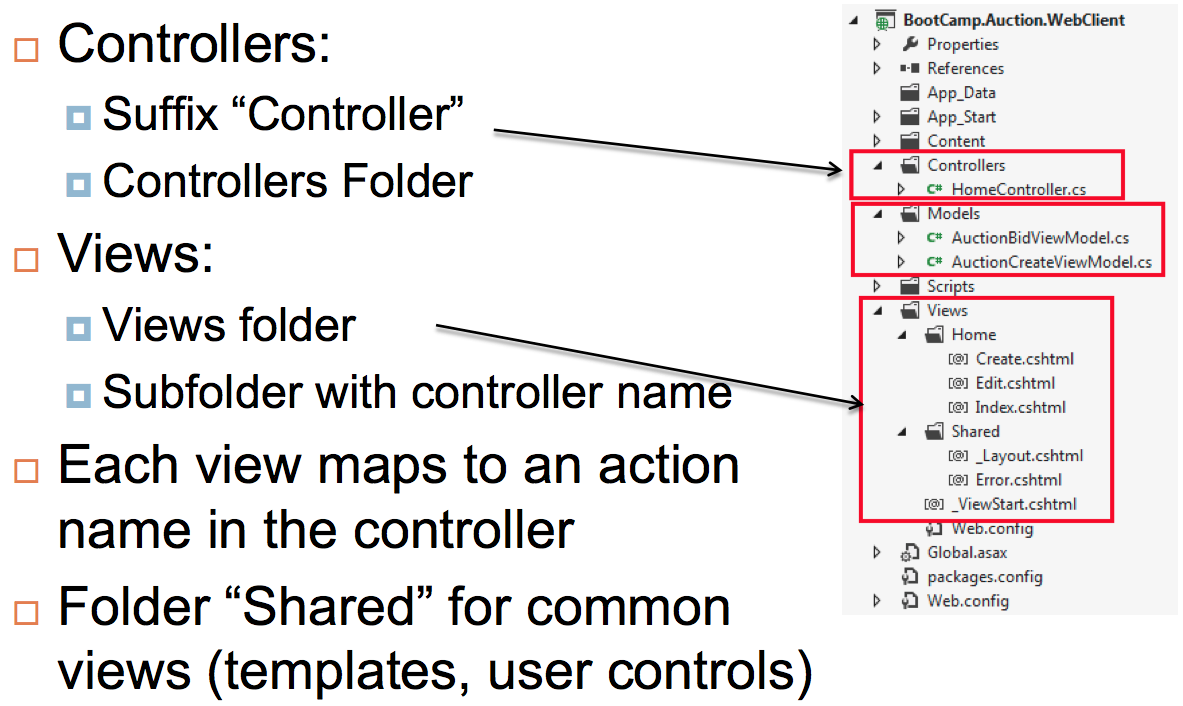
\includegraphics[scale=0.3]{mvc.png}
\end{center}
\subsection{Controllers}
\begin{itemize}
	\item Controllers handle all incoming requests
	\item Retrieve data from storage
	\item Store posted data in storage (http post)
	\item Pass the data to a View to generate the HTML/CSS/JavaScript for display
	\item Controllers can implement REST APIs (derive controller from ApiController)
\end{itemize}
\subsubsection{Actions}
The simplest controller just returns HTML to the Web browser \\
IMPORTANT: By default, all public methods in a controller class can be called from the Web browser \\
Controllers can easily be tested (without ASP.NET runtime) \\
Most controller methods return a type of action results:
\begin{center}
	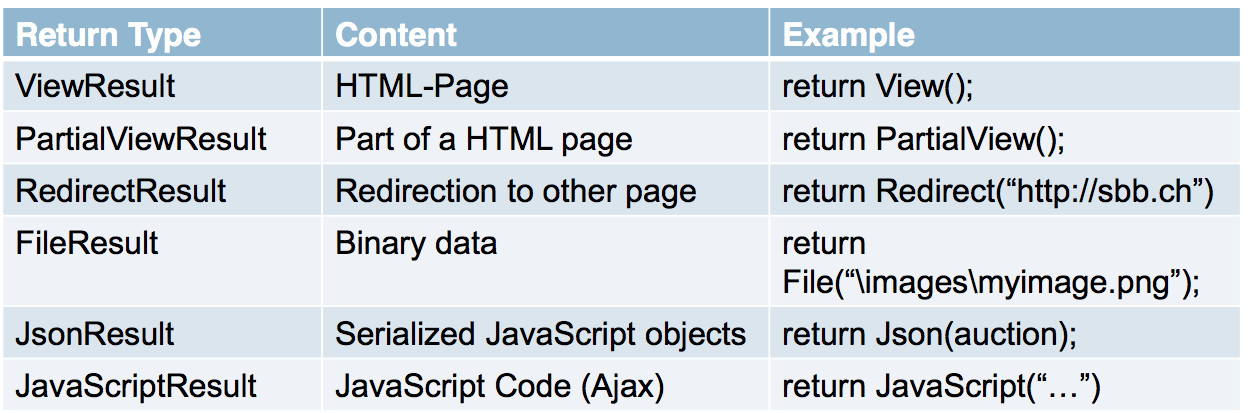
\includegraphics[scale=0.3]{mvc_controller_actions.png}
\end{center}
\subsubsection{Ajax}
Ajax calls can also be handled by the controller
\begin{lstlisting}[language=Java, caption=Ajax:, style=JavaStyle]
// View
@Ajax.ActionLink("Click me", "Click", null)

// Controller
public JavaScriptResult Click() {
   return JavaScript("alert('Hallo World');");
}
\end{lstlisting}
\subsubsection{View typed}
Typed way to passed data to the View:
\begin{lstlisting}[language=Java, caption=typed view:, style=JavaStyle]
// Controller
public ActionResult Index() {
      return View(db.Item.ToList());
}

// View
@model IEnumerable<Auction.Models.Item> Html.DisplayNameFor(model => model.StartPrice)
\end{lstlisting}
\subsubsection{View untyped}
The ViewBag is used to push untyped data to the view (Properties are created at runtime...)
\begin{lstlisting}[language=Java, caption=typed view:, style=JavaStyle]
// Controller
ViewBag.Persons = new SelectList(context.People, "Id", "Name");

// View
@Html.DropDownListFor(model => model.SellerId, (SelectList)ViewBag.Persons)
\end{lstlisting}
\subsection{Views}
\subsubsection{Code Blocks	}
\begin{center}
	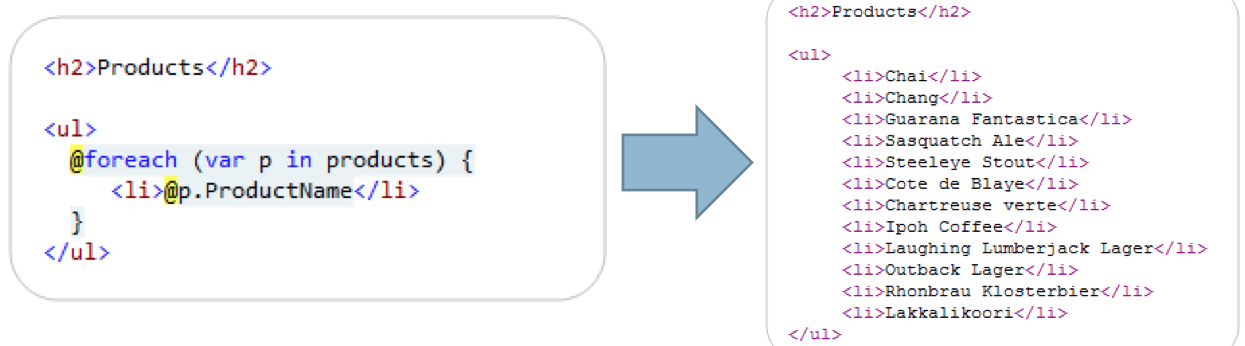
\includegraphics[scale=0.3]{mvc_views_at.png}
\end{center}
\begin{center}
	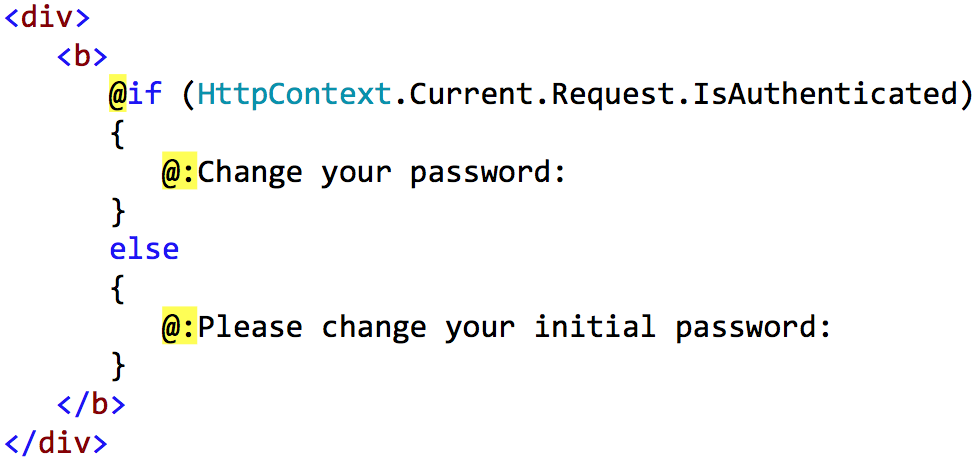
\includegraphics[scale=0.2]{mvc_views_at_break.png}
\end{center}
\subsubsection{HtmlHelpers}
\begin{lstlisting}[language=Java, caption=typed view:, style=JavaStyle]
// <a href="/Home/Edit/3">Edit Record</a>
@Html.ActionLink("Edit Record", "Edit", new {Id=3}):

// <label for="FirstName">FirstName</label>
@Html.LabelFor(model => model.FirstName):

// <input class="text-box single-line" data-val="true" data-val-required="The FirstName field is required." id="FirstName" name="FirstName" type="text" value="" />
@Html.EditorFor(model => model.FirstName):
\end{lstlisting}
\subsubsection{Layout Pages}
\begin{center}
	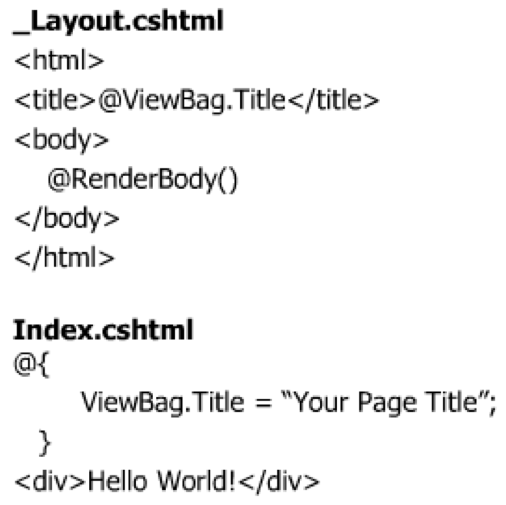
\includegraphics[scale=0.2]{mvc_view_layout.png}
\end{center}
\subsection{Routes}
\begin{lstlisting}[language=Java, caption=routes, style=JavaStyle]
routes.MapRoute(
	"Default", // Route name
	"{controller}/{action}/{id}", // URL with parameters
	new { controller = "Home", action = "Index", id = UrlParameter.Optional } // Default
);
\end{lstlisting}
\subsection{Model}
Validations can be specified for individual fields in the data model. Client and Server validation with no additional coding.	
\begin{center}
	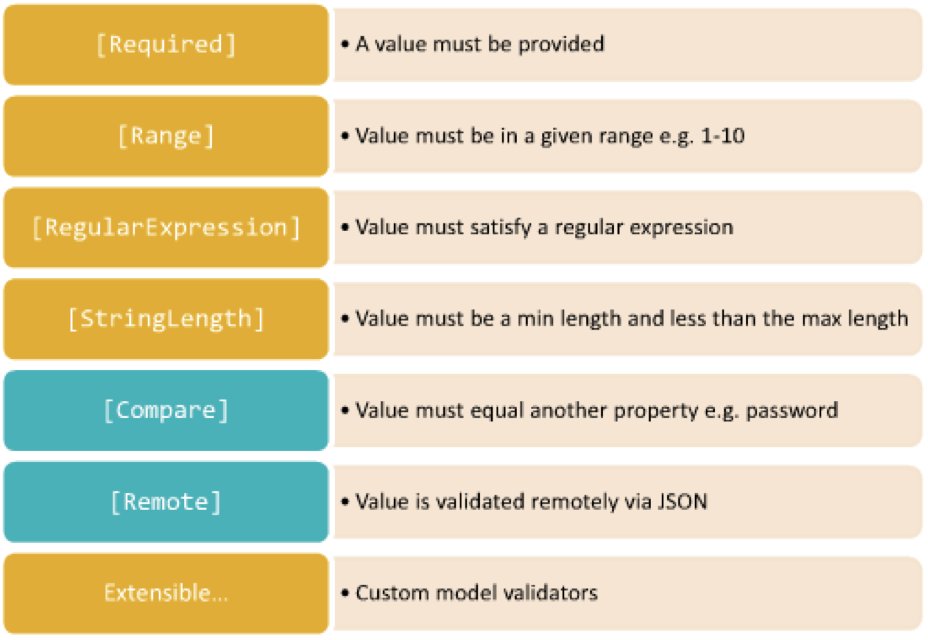
\includegraphics[scale=0.2]{mvc_model.png}
\end{center}

\pagebreak
\section{Codebeispiele}
\subsection{WPF XAML}
\begin{lstlisting}[ language=Java, caption=MainWindow.xaml, style=JavaStyle]
<Window x:Class="Fhnw.Dnead.Auction.WpfClient.Views.MainWindow"
        xmlns="http://schemas.microsoft.com/winfx/2006/xaml/presentation"
        xmlns:x="http://schemas.microsoft.com/winfx/2006/xaml"
        Title="MainWindow" Height="350" Width="596.317"
    xmlns:my="clr-namespace:Fhnw.Dnead.Auction.WpfClient"
    xmlns:conv="clr-namespace:Fhnw.Dnead.Auction.WpfClient.Converter">

    <Window.Resources>
        <conv:BooleanToStatusTextConverter x:Key="booleanToStatusTextConverter" />
        <BooleanToVisibilityConverter x:Key="booleanToVisibilityConverter" />
    </Window.Resources>
    
    <Grid>
        <DataGrid AutoGenerateColumns="False" Name="dgAuctionItems" ItemsSource="{Binding Path=Auctions}" Margin="0,48,0,0" IsReadOnly="True">
            <DataGrid.Columns>
                    <DataGridTemplateColumn>
                        <DataGridTemplateColumn.CellTemplate>
                            <DataTemplate>
                            <Button Background="Red" Name="btnBuy" Content="Buy" Width="44" Margin="2" Visibility="{Binding Path=Open, Converter={StaticResource booleanToVisibilityConverter}}" IsCancel="False" Click="BtnBuyClick"></Button>
                            </DataTemplate>
                        </DataGridTemplateColumn.CellTemplate>
                    </DataGridTemplateColumn>
                    <DataGridTextColumn Binding="{Binding Path=Name}" Header="Artikel" />
                <DataGridTextColumn Binding="{Binding Path=StartPrice}" Header="Start Preis" />
                <DataGridTextColumn Binding="{Binding Path=Bid}" Header="Aktuelles Gebot" />
                <DataGridTextColumn Binding="{Binding Path=StartTime}" Header="Auktionsstart" />
                <DataGridTextColumn Binding="{Binding Path=EndTime}" Header="Auktionsende" />
                <DataGridTextColumn Binding="{Binding Path=Seller}" Header="Verk{\a}ufer" />
                <DataGridTextColumn Binding="{Binding Path=Buyer}" Header="K{\a}ufer" />
                <DataGridTextColumn Binding="{Binding Path=Open, Converter={StaticResource booleanToStatusTextConverter}}" Header="Status" />
                <DataGridTemplateColumn Header="Bild">
                    <DataGridTemplateColumn.CellTemplate>
                        <DataTemplate>
                            <Image Source="{Binding Path=Picture}" Width="64" Height="64" />
                        </DataTemplate>
                    </DataGridTemplateColumn.CellTemplate>
                </DataGridTemplateColumn>

            </DataGrid.Columns>
        </DataGrid>
        <Button Content="Artikel verkaufen" HorizontalAlignment="Left" Margin="23,10,0,0" VerticalAlignment="Top" Width="162" Click="BtnSellClick"/>

    </Grid>
</Window>
\end{lstlisting}

\begin{lstlisting}[ language=Java, caption=BidView.xaml, style=JavaStyle]
<Window x:Class="Fhnw.Dnead.Auction.WpfClient.Views.BidView"
        xmlns="http://schemas.microsoft.com/winfx/2006/xaml/presentation"
        xmlns:x="http://schemas.microsoft.com/winfx/2006/xaml"
        Title="Bieten" Height="176" Width="300">
   
    <DockPanel>
        <StackPanel Orientation="Horizontal" DockPanel.Dock="Bottom" HorizontalAlignment="Right">
            <Button Content="Cancel" Height="23" HorizontalAlignment="Left" Margin="10"  Name="btnCancel" VerticalAlignment="Bottom" Width="75" IsCancel="True" />
            <Button Content="OK" Height="23" HorizontalAlignment="Left" Margin="10"  Name="btnOk" VerticalAlignment="Bottom" Width="75" Command="{Binding OkCommand}" CommandParameter="{Binding RelativeSource={RelativeSource FindAncestor, AncestorType={x:Type Window}}}"/>
        </StackPanel>
        <StackPanel Orientation="Horizontal" HorizontalAlignment="Right" DockPanel.Dock="Bottom">
            <TextBlock Height="23" HorizontalAlignment="Right" Margin="10" Text="Gebot" VerticalAlignment="Bottom" />
            <TextBox Height="24" Margin="10" HorizontalAlignment="Stretch" Width="100" Name="txtBid" VerticalAlignment="Bottom" Text="{Binding Path=Bid}"/>
        </StackPanel>
        <Viewbox Margin="10" >
            <Image Name="imgPicture" Source="{Binding Path=Item.Picture}">

            </Image>
        </Viewbox>
    </DockPanel>
</Window>
\end{lstlisting}

\begin{lstlisting}[ language=Java, caption=MainViewModel.cs, style=JavaStyle]
using System;
using System.Collections.ObjectModel;
using System.Linq;
using System.Windows.Threading;
using Fhnw.Dnead.Auction.DAL;

namespace Fhnw.Dnead.Auction.WpfClient.ViewModels
{
    public class MainViewModel : ViewModelBase
    {
        readonly ObservableCollection<AuctionViewModel> auctions = new ObservableCollection<AuctionViewModel>();

        public ObservableCollection<AuctionViewModel> Auctions
        {
            get
            {
                return auctions;
            }
        }

        readonly AuctionContext context = new AuctionContext();

        /// <summary>
        /// Timer to detect auction closes
        /// </summary>
        readonly DispatcherTimer auctionTimer = new DispatcherTimer();


        private void StartAuctionTimer()
        {
            auctionTimer.Tick +=
                delegate
                    {
                        // set all timed out auctions to closed
                        UpdateAuctionOpenStatus();
                        context.SaveChanges();
                    };

            auctionTimer.Interval = new TimeSpan(0, 0, 1);
            auctionTimer.Start();
        }

        /// <summary>
        /// Verifies expiration date of auctions and updates open status if expired.
        /// </summary>
        private void UpdateAuctionOpenStatus()
        {
            auctions.Where(a => a.EndTime < DateTime.Now).ToList().ForEach(a => a.Open = false);
        }

        public MainViewModel()
        {
            // read existing data from db and fill them in the observable collection
            context.Auctions.ToList().ForEach(a => auctions.Add(new AuctionViewModel { Auction = a }));

            StartAuctionTimer();

        }

        public void AddNewAuction(AuctionViewModel newAuctionEntity)
        {
            context.Auctions.Add(newAuctionEntity.Auction);
            context.SaveChanges();
            Auctions.Add(newAuctionEntity)
\end{lstlisting}

\begin{lstlisting}[ language=Java, caption=BidViewModel.cs, style=JavaStyle]
using System;
using System.Windows;
using System.Windows.Input;
using Fhnw.Dnead.Auction.WpfClient.Commands;


namespace Fhnw.Dnead.Auction.WpfClient.ViewModels
{
    /// <summary>
    /// ViewModel for a bid for an auction.
    /// </summary>
    class BidViewModel : ViewModelBase
    {
        private DelegateCommand<Window> okCommand;

        public string Bid { get; private set; }
        private readonly AuctionViewModel item;

        public BidViewModel(AuctionViewModel item)
        {
            this.item = item;
            Bid = ((item.Bid == 0 || item.Bid == null? item.StartPrice : item.Bid) + 1).ToString();
        }

        public bool ValidateEntries()
        {
            int newBid;
            if (!int.TryParse(Bid, out newBid)) return false;
            if (newBid == 0) return false;
            if (newBid <= item.Bid) return false;
            if (newBid <= item.StartPrice) return false;

            item.Bid = newBid;
            item.Buyer = Environment.UserName;

            return true;
        }

        public ICommand OkCommand
        {
            get
            {
                if (okCommand == null)
                {
                    okCommand = new DelegateCommand<Window>(DoOk, CanDoOk);
                }
                return okCommand;
            }
        }

        void DoOk(Window win)
{
            if (ValidateEntries())
            {
                win.DialogResult = true;
            }
}

        bool CanDoOk(Window win) { return true; }
    }
}
\end{lstlisting}

% Inhalt Ende 
\end{document} 